\documentclass[11pt]{article}
\usepackage[utf8]{inputenc}
\usepackage[T1]{fontenc}
\usepackage[a4paper,margin=2.2cm,top=2.6cm]{geometry}
\usepackage{amsmath,amssymb}
\usepackage{graphicx}
\usepackage{enumitem}
\usepackage{xcolor}
\usepackage[most]{tcolorbox}
\usepackage{fancyhdr}
\usepackage[some]{background}
\usepackage{icomma}
\usepackage{tikz}
\usepackage{siunitx}

\definecolor{itbblue}{RGB}{0,86,167}
\definecolor{navyhead}{RGB}{16,46,96}
\definecolor{gold}{RGB}{233,170,40}
\definecolor{soalbg}{RGB}{225,236,248}

\pagestyle{fancy}\fancyhf{}
\lhead{\small\scshape Fisika -- SSU ITB 2023}
\chead{\small www.tiktok.com/@result\_han}
\rhead{\small @result\_han}
\cfoot{\small\thepage}
\renewcommand{\headrulewidth}{0.4pt}

\backgroundsetup{scale=6,color=black!7,opacity=0.7,angle=45,
  position=current page.center,contents={@result\_han}}

\newtcolorbox{soalbox}[2]{breakable,colback=soalbg,colframe=itbblue,
  coltitle=white,fonttitle=\bfseries\sffamily,title={Soal #1.\ #2},
  boxrule=0.8pt,arc=3pt,left=3mm,right=3mm,top=2mm,bottom=2mm}
\newtcolorbox{pembox}[1]{breakable,colback=white,colframe=navyhead,
  coltitle=white,fonttitle=\bfseries\sffamily,title={Pembahasan Soal #1},
  boxrule=0.8pt,arc=3pt,left=3mm,right=3mm,top=2mm,bottom=2mm}

\newenvironment{pil}{\begin{enumerate}[label=\textbf{\Alph*.},leftmargin=*,itemsep=1pt,topsep=3pt]}{\end{enumerate}}
\newcommand{\jw}[1]{\par\smallskip\noindent\textbf{Jawaban: #1}}
\newcommand{\fig}[2][0.55\textwidth]{\begin{center}\includegraphics[width=#1]{#2}\end{center}}

\linespread{1.04}
\begin{document}

%================= SAMPUL =================
\thispagestyle{empty}
\noindent\begin{tikzpicture}
\fill[itbblue](0,0)rectangle(\textwidth,-3.4);
\fill[navyhead](0,-3.4)rectangle(\textwidth,-3.55);
\fill[gold](0,-3.55)rectangle(\textwidth,-3.68);
\node[anchor=north west,text=white,font=\sffamily\bfseries\small]at(0.4,-0.4){SOAL ASLI DAN PEMBAHASAN};
\node[anchor=north west,text=white,font=\sffamily\bfseries\LARGE]at(0.4,-0.75){SELEKSI MANDIRI ITB 2023};
\node[anchor=north west,text=white,font=\sffamily\bfseries\LARGE]at(0.4,-1.45){BIDANG FISIKA};
\node[anchor=north west,text=white!90,font=\sffamily\footnotesize]at(0.4,-2.15){Formatting dan pengetikan ulang oleh @result\_han};
\node[anchor=north west,text=white!90,font=\sffamily\footnotesize]at(0.4,-2.5){Follow TikTok: www.tiktok.com/@result\_han};
\node[anchor=north west,text=white!90,font=\sffamily\footnotesize]at(0.4,-2.85){Beli paket soal PTN lainnya: lynk.id/result\_han};
\node[anchor=north east,fill=white,inner sep=2pt]at(\textwidth-0.3,-0.35){\includegraphics[height=1.9cm]{images/8/8-1.png}};
\end{tikzpicture}
\vspace{2.4cm}
\begin{center}
\begin{tcolorbox}[width=0.72\textwidth,colback=soalbg!50,colframe=itbblue,arc=4pt]
{\Large\bfseries Ringkasan Paket}\\[0.4em]
30 soal pilihan ganda SSU ITB 2023 bidang Fisika\\
Format: Soal -- Pembahasan -- Soal -- Pembahasan\\
Pembahasan bertahap: konsep, persamaan, substitusi, dan pilihan jawaban\\
Disusun ulang dengan tata letak LaTeX yang rapi untuk belajar mandiri\\[0.6em]
\rule{\linewidth}{0.3pt}\\[0.4em]
{\small Catatan: dokumen ini adalah hasil pengetikan ulang dan pembahasan edukatif. Gunakan pembahasan untuk memahami konsep, bukan sekadar menghafal opsi.}\\[0.6em]
\hfill\textbf{@result\_han}
\end{tcolorbox}
\end{center}
\vfill
\begin{center}\small\textbf{www.tiktok.com/@result\_han}\quad|\quad\textbf{lynk.id/result\_han}\end{center}
\clearpage

\begin{center}{\Large\bfseries Soal dan Pembahasan Fisika}\\[0.2em]
{\small Seleksi Mandiri ITB 2023 -- Bidang Fisika}\end{center}
\medskip

\begin{soalbox}{1}{Gerak Parabola}
Pada saat $t=0$ s, sebuah meriam menembakkan peluru ke udara sehingga peluru bergerak mengikuti lintasan gerak parabola. Pada saat $2{,}5$ s, posisi peluru tersebut berada pada $10$ m arah horizontal dan $40$ m arah vertikal dihitung dari posisi awal peluru ditembakkan. Jika percepatan gravitasi adalah $10$ m/s$^2$, peluru jatuh di tanah pada jarak $\ldots$ m dari posisi meriam.
\begin{pil}\item $42{,}80$ \item $35{,}60$ \item $16{,}40$ \item $62{,}80$ \item $22{,}80$\end{pil}
\end{soalbox}
\begin{pembox}{1}
Pisahkan gerak horizontal dan vertikal. Dari posisi horizontal saat $t=2{,}5$ s: $x=v_{0x}t\Rightarrow 10=v_{0x}(2{,}5)\Rightarrow v_{0x}=4$ m/s. Untuk arah vertikal $y=v_{0y}t-\tfrac12gt^2$: $40=2{,}5v_{0y}-\tfrac12(10)(2{,}5)^2=2{,}5v_{0y}-31{,}25\Rightarrow v_{0y}=28{,}5$ m/s. Peluru kembali ke tanah ketika $y=0$: $0=t(v_{0y}-5t)$, sehingga $t=\tfrac{28{,}5}{5}=5{,}7$ s. Jarak horizontal total $R=v_{0x}t=4(5{,}7)=22{,}8$ m.
\jw{E}
\end{pembox}

\begin{soalbox}{2}{Kecepatan Sesaat}
Suatu benda bergerak sepanjang sumbu $x$ menurut persamaan $x(t)=4t^2-2t+3$ m. Kecepatan sesaat pada $t=4$ s adalah $\ldots$ m/s.
\begin{pil}\item $-16$ \item $24$ \item $65$ \item $0$ \item $30$\end{pil}
\end{soalbox}
\begin{pembox}{2}
Kecepatan sesaat adalah turunan pertama posisi: $v(t)=\dfrac{dx}{dt}=8t-2$. Pada $t=4$ s: $v(4)=8(4)-2=30$ m/s.
\jw{E}
\end{pembox}

\begin{soalbox}{3}{Gerak Dua Dimensi}
Benda A dan B bergerak dalam ruang dua dimensi $x$-$y$. Benda A bergerak sepanjang lintasan dengan $x_A(t)=(t+2)(t-5)$ m dan $y_A(t)$ berupa garis lurus dari $y=-5$ m pada $t=0$ s sampai $y=60$ m pada $t=1$ s. Komponen $x$ dan $y$ dari kecepatan benda B berturut-turut adalah $v$ m/s dan $-5+20t$ m/s. Pada saat $t=0$ s, kedua benda berada di tempat yang sama. Kedua benda dapat bertemu kembali apabila $v=\ldots$ m/s.
\begin{pil}\item $4$ \item $8$ \item $7$ \item $5$ \item $6$\end{pil}
\end{soalbox}
\begin{pembox}{3}
Posisi awal A: $x_A(0)=(2)(-5)=-10$ m, sehingga posisi awal B juga $(-10,-5)$. Untuk A, $y_A$ berubah lurus dari $-5$ ke $60$ dalam 1 s: $y_A(t)=-5+65t$. Untuk B, $v_{By}=-5+20t$, maka $y_B(t)=-5+\int_0^t(-5+20\tau)\,d\tau=-5-5t+10t^2$. Saat bertemu, $y_A=y_B$: $-5+65t=-5-5t+10t^2\Rightarrow 70t=10t^2\Rightarrow t=7$ s. Pada saat ini $x_A(7)=(9)(2)=18$ m. Untuk B, $x_B(t)=-10+vt$, sehingga $-10+7v=18\Rightarrow v=4$ m/s.
\jw{A}
\end{pembox}

\begin{soalbox}{4}{Percepatan pada Lintasan Kurva}
Suatu partikel bergerak pada bidang $x$-$y$ dengan lintasan yang dinyatakan oleh fungsi $y(x)=(2x+6)(x-3)$ m. Apabila komponen $x$ dari kecepatan partikel bernilai tetap, yaitu $0{,}75$ m/s, maka komponen $y$ dari percepatan partikel sama dengan $\ldots$ m/s$^2$.
\begin{pil}\item $3{,}00$ \item $1{,}125$ \item $2{,}25$ \item $1{,}50$ \item $0{,}56$\end{pil}
\end{soalbox}
\begin{pembox}{4}
Uraikan lintasan: $y=(2x+6)(x-3)=2x^2-18$, sehingga $\dfrac{dy}{dx}=4x$. Komponen kecepatan vertikal $v_y=\dfrac{dy}{dt}=\dfrac{dy}{dx}\dfrac{dx}{dt}=4xv_x$. Dengan $v_x=0{,}75$: $v_y=3x$. Percepatan vertikal $a_y=\dfrac{dv_y}{dt}=3\dfrac{dx}{dt}=3(0{,}75)=2{,}25$ m/s$^2$.
\jw{C}
\end{pembox}

\begin{soalbox}{5}{Kecepatan Rata-Rata}
Posisi suatu partikel yang bergerak di sepanjang sumbu $x$ dinyatakan oleh fungsi posisi $x(t)=t(b-ct)$, dengan $b=20$ m/s dan $c=1$ m/s$^2$. Kecepatan rata-rata partikel tersebut dalam selang waktu dari $t_1=0$ hingga $t_2=4$ s adalah $\ldots$ m/s.
\begin{pil}\item $28$ \item $16$ \item $20$ \item $12$ \item $24$\end{pil}
\end{soalbox}
\begin{pembox}{5}
$\bar v=\dfrac{x(t_2)-x(t_1)}{t_2-t_1}$. Fungsi posisi $x(t)=bt-ct^2$. $x(0)=0$ dan $x(4)=20(4)-1(4)^2=80-16=64$ m. Maka $\bar v=\dfrac{64-0}{4-0}=16$ m/s.
\jw{B}
\end{pembox}

\begin{soalbox}{6}{Percepatan dari Fungsi Posisi}
Benda A dan benda B bergerak sepanjang sumbu $x$. Posisi benda A pada saat $t$ dinyatakan oleh $x(t)=(t+2)(t-5)(t+7)$ m, sedangkan kecepatan benda B diberikan oleh $v(t)=-5+44t$ m/s. Maka posisi benda A ketika percepatannya sama dengan percepatan benda B adalah di $x=\ldots$ m.
\begin{pil}\item $94$ \item $114$ \item $84$ \item $104$ \item $124$\end{pil}
\end{soalbox}
\begin{pembox}{6}
Percepatan benda B: $a_B=\dfrac{dv_B}{dt}=44$ m/s$^2$. Untuk benda A, $x_A(t)=(t+2)(t-5)(t+7)$. Uraikan $(t+2)(t-5)=t^2-3t-10$, sehingga $x_A(t)=t^3+4t^2-31t-70$. Maka $v_A(t)=3t^2+8t-31$ dan $a_A(t)=6t+8$. Saat percepatan sama: $6t+8=44\Rightarrow t=6$ s. Posisi A: $x_A(6)=(8)(1)(13)=104$ m.
\jw{D}
\end{pembox}

\begin{soalbox}{7}{Dinamika pada Bidang Miring}
Dua buah balok bermassa $m_1=4$ kg dan $m_2=5$ kg terikat pada tali yang melalui sebuah katrol. Kedua balok berada pada permukaan bidang miring licin. Balok $m_1$ berada pada bidang $45^\circ$, sedangkan balok $m_2$ berada pada bidang $30^\circ$. Apabila balok $m_2$ ditarik dengan gaya konstan $F=20$ N sejajar bidang ke arah bawah bidang, dan $g=10$ m/s$^2$, maka besar percepatan balok $m_1$ adalah $\ldots$ m/s$^2$.
\fig[0.5\textwidth]{images/8/8-2.png}
\begin{pil}\item $2{,}59$ \item $3{,}89$ \item $3{,}70$ \item $1{,}86$ \item $3{,}93$\end{pil}
\end{soalbox}
\begin{pembox}{7}
Bidang licin, sehingga gaya sepanjang bidang hanya berasal dari komponen berat, tegangan tali, dan gaya luar $F$. Ambil arah positif: $m_2$ bergerak turun pada bidang $30^\circ$, sehingga $m_1$ naik pada bidang $45^\circ$. Gaya penggerak pada $m_2$: $F+m_2g\sin30^\circ=20+5(10)(0{,}5)=45$ N. Gaya yang menahan adalah komponen berat $m_1$: $m_1g\sin45^\circ=4(10)\left(\tfrac{\sqrt2}{2}\right)=20\sqrt2\approx28{,}28$ N. Gaya resultan sistem $F_{\text{net}}=45-28{,}28=16{,}72$ N, massa total $m_1+m_2=9$ kg. Maka $a=\dfrac{16{,}72}{9}=1{,}86$ m/s$^2$.
\jw{D}
\end{pembox}

\begin{soalbox}{8}{Gaya Gesek Statis Maksimum}
Sebuah balok bermassa $40$ kg berada pada meja horizontal kasar dihubungkan dengan sebuah drum kosong bermassa $2$ kg menggunakan seutas tali melalui katrol licin dan ringan. Koefisien gesek statis dan kinetis antara balok dan meja masing-masing adalah $0{,}35$ dan $0{,}25$. Jika sejumlah air dengan massa jenis $1000$ kg/m$^3$ dimasukkan ke dalam drum dan $g=10$ m/s$^2$, berapakah volume maksimum air dalam drum agar sistem tetap tidak bergerak?
\fig[0.5\textwidth]{images/8/8-3.png}
\begin{pil}\item $12$ liter \item $16$ liter \item $20$ liter \item $39{,}3$ liter \item $8$ liter\end{pil}
\end{soalbox}
\begin{pembox}{8}
Agar sistem tetap diam, tegangan tali akibat berat drum berisi air tidak boleh melebihi gaya gesek statis maksimum: $f_{s,\max}=\mu_sN$. Karena balok di meja horizontal, $N=m_bg=40(10)=400$ N, sehingga $f_{s,\max}=0{,}35(400)=140$ N. Drum dan air menggantung memberikan berat $W=(m_d+m_{\text{air}})g$. Agar tepat maksimum, $(2+m_{\text{air}})(10)=140\Rightarrow m_{\text{air}}=12$ kg. Volume air $V=\dfrac{m}{\rho}=\dfrac{12}{1000}=0{,}012$ m$^3=12$ liter.
\jw{A}
\end{pembox}

\begin{soalbox}{9}{Gaya Tarik dan Gesekan}
Sebuah balok dengan massa $m=2$ kg diberi gaya konstan sebesar $F=20$ N yang membentuk sudut $\theta$ terhadap sumbu $x$ positif. Jika $\tan\theta=3/4$, koefisien gesek statis dan kinetis antara balok dan meja masing-masing $0{,}3$ dan $0{,}2$, serta $g=10$ m/s$^2$, besar percepatan balok adalah $\ldots$ m/s$^2$.
\fig[0.5\textwidth]{images/8/8-4.png}
\begin{pil}\item $3{,}20$ \item $4{,}80$ \item $6{,}80$ \item $5{,}00$ \item $6{,}00$\end{pil}
\end{soalbox}
\begin{pembox}{9}
Dari $\tan\theta=3/4$, segitiga komponen gaya memiliki perbandingan sisi $3:4:5$, sehingga $\cos\theta=\tfrac45$ dan $\sin\theta=\tfrac35$. Gaya menekan balok, sehingga komponen vertikalnya menambah gaya normal. Komponen gaya: $F_x=F\cos\theta=20\left(\tfrac45\right)=16$ N, $F_y=F\sin\theta=20\left(\tfrac35\right)=12$ N. Gaya normal $N=mg+F_y=2(10)+12=32$ N. Gesek statis maksimum $f_{s,\max}=0{,}3(32)=9{,}6$ N. Karena $F_x=16>9{,}6$ N, balok bergerak; gesek kinetis $f_k=0{,}2(32)=6{,}4$ N. Resultan horizontal $\Sigma F_x=16-6{,}4=9{,}6$ N. Maka $a=\dfrac{9{,}6}{2}=4{,}8$ m/s$^2$.
\jw{B}
\end{pembox}

\begin{soalbox}{10}{Dua Balok Bertumpuk}
Sebuah balok A dengan massa $20$ kg ditempatkan pada meja horizontal licin dan mendapat gaya horizontal konstan $F$ ke arah kanan sehingga bergerak dengan percepatan $6$ m/s$^2$ relatif terhadap meja. Balok B dengan massa $20$ kg bergeser pada permukaan atas balok A dengan percepatan $4$ m/s$^2$ yang juga ke arah kanan relatif terhadap meja. Jika $g=10$ m/s$^2$ dan koefisien gesek antara balok A dan B adalah $0{,}4$, maka nilai gaya $F=\ldots$ N.
\fig[0.5\textwidth]{images/8/8-5.png}
\begin{pil}\item $360$ \item $200$ \item $260$ \item $280$ \item $160$\end{pil}
\end{soalbox}
\begin{pembox}{10}
Karena balok B bergeser relatif terhadap A, gaya gesek antara A dan B adalah gesek kinetis $f_k=\mu N=\mu m_Bg=0{,}4(20)(10)=80$ N. Gaya ini mempercepat B: $a_B=\dfrac{f_k}{m_B}=\dfrac{80}{20}=4$ m/s$^2$, sesuai informasi soal. Pada balok A, gaya $F$ menarik ke kanan dan gesekan dari B bekerja ke kiri sebesar $80$ N: $F-80=m_Aa_A=20(6)=120$, sehingga $F=200$ N.
\jw{B}
\end{pembox}

\begin{soalbox}{11}{Teorema Usaha-Energi dalam Vektor}
Saat $t=0$, sebuah gaya konstan $\vec F=(-5\hat i+2\hat j+3\hat k)$ N mulai bekerja pada partikel bermassa $2$ kg yang sedang bergerak lurus dengan kelajuan $3$ m/s. Kelajuan partikel ketika mengalami perpindahan $\vec d=(2\hat i+5\hat j+\hat k)$ m dari titik awalnya adalah $\ldots$ m/s.
\begin{pil}\item $4{,}31$ \item $4{,}58$ \item $3{,}46$ \item $3{,}24$ \item $3{,}12$\end{pil}
\end{soalbox}
\begin{pembox}{11}
Usaha oleh gaya konstan $W=\vec F\cdot\vec d=(-5)(2)+(2)(5)+(3)(1)=-10+10+3=3$ J. Energi kinetik awal $K_i=\tfrac12mv_i^2=\tfrac12(2)(3^2)=9$ J. Menurut teorema usaha-energi $K_f=K_i+W=9+3=12$ J. Karena $K_f=\tfrac12mv_f^2$: $12=\tfrac12(2)v_f^2\Rightarrow v_f^2=12\Rightarrow v_f=\sqrt{12}=3{,}46$ m/s.
\jw{C}
\end{pembox}

\begin{soalbox}{12}{Usaha oleh Gaya Berubah}
Sebuah gaya $\vec F(x)=x(k-x)\hat i$ bekerja pada suatu partikel yang sedang bergerak sepanjang sumbu $x$. Gaya $F$ dalam satuan Newton, $x$ dalam satuan meter, dan $k$ adalah suatu konstanta. Ketika berada pada posisi $x=0$ m, energi kinetik partikel adalah $19$ J. Ketika mencapai posisi $x=3$ m, energi kinetik partikel adalah $10$ J. Nilai konstanta $k$ adalah $\ldots$ N/m.
\begin{pil}\item $4{,}00$ \item $0{,}50$ \item $0$ \item $3{,}00$ \item $1{,}00$\end{pil}
\end{soalbox}
\begin{pembox}{12}
Untuk gaya yang berubah, $W=\displaystyle\int_{x_1}^{x_2}F(x)\,dx$. Menurut teorema usaha-energi $W=K_f-K_i=10-19=-9$ J. Dengan $F(x)=kx-x^2$: $W=\int_0^3(kx-x^2)\,dx=\left[\tfrac{kx^2}{2}-\tfrac{x^3}{3}\right]_0^3=\tfrac{9k}{2}-9$. Karena $W=-9$: $\tfrac{9k}{2}-9=-9\Rightarrow\tfrac{9k}{2}=0\Rightarrow k=0$.
\jw{C}
\end{pembox}

\begin{soalbox}{13}{Usaha Gaya Nonkonservatif}
Sebuah balok bermassa $2{,}5$ kg meluncur sejauh $1$ m pada lintasan lurus dengan kemiringan $\alpha$ terhadap bidang datar, dengan $\tan\alpha=3/4$. Koefisien gesek statis dan kinetis antara balok dan permukaan lintasan masing-masing $0{,}50$ dan $0{,}20$. Jika $g=10$ m/s$^2$, usaha yang dilakukan gaya nonkonservatif adalah $\ldots$ J.
\begin{pil}\item $5{,}00$ \item $4{,}00$ \item $-5{,}00$ \item $-3{,}00$ \item $-4{,}00$\end{pil}
\end{soalbox}
\begin{pembox}{13}
Gaya nonkonservatif di sini adalah gaya gesek kinetis karena balok meluncur. Dari $\tan\alpha=3/4$: $\sin\alpha=\tfrac35$, $\cos\alpha=\tfrac45$. Gaya normal $N=mg\cos\alpha=2{,}5(10)\left(\tfrac45\right)=20$ N. Gesek kinetis $f_k=\mu_kN=0{,}20(20)=4$ N. Karena arah gesek berlawanan dengan arah gerak, usahanya negatif: $W_{\text{gesek}}=-f_ks=-4(1)=-4$ J.
\jw{E}
\end{pembox}

\begin{soalbox}{14}{Grafik Percepatan dan Gaya}
Dua buah gaya $F_1$ dan $F_2$ bekerja pada sebuah benda bermassa $1{,}5$ kg di lantai datar tanpa gesekan. Besar gaya $F_1$ tetap dengan arah membentuk sudut $\theta$ terhadap sumbu $x$ yang dapat diubah. Gaya $F_2$ tetap dan searah sumbu $x$. Grafik menunjukkan bahwa nilai $a_x$ pada $\theta=0^\circ$ adalah $A=3$ m/s$^2$, sedangkan pada $\theta=90^\circ$ nilai $a_x=A/3$. Besar gaya $F_2$ adalah $\ldots$ N.
\fig[0.7\textwidth]{images/8/8-6.png}
\begin{pil}\item $3{,}50$ \item $0{,}50$ \item $1{,}50$ \item $4{,}50$ \item $3{,}00$\end{pil}
\end{soalbox}
\begin{pembox}{14}
Komponen gaya arah $x$: $\Sigma F_x=F_1\cos\theta+F_2$. Dengan hukum II Newton $a_x=\dfrac{F_1\cos\theta+F_2}{m}$. Saat $\theta=90^\circ$, komponen $x$ dari $F_1$ nol karena $\cos90^\circ=0$, sehingga $a_x(90^\circ)=\dfrac{F_2}{m}$. Dari grafik $a_x(90^\circ)=\dfrac{A}{3}=\dfrac33=1$ m/s$^2$. Maka $F_2=ma_x=1{,}5(1)=1{,}5$ N.
\jw{C}
\end{pembox}

\begin{soalbox}{15}{Tegangan Tali pada Dua Balok}
Sebuah benda A bermassa $2$ kg dan benda B bermassa $6$ kg berada pada permukaan meja horizontal licin dan dihubungkan dengan sebuah tali tak bermassa. Gaya $F_A=10{,}0$ N dengan sudut $30^\circ$ terhadap sumbu $x$ bekerja pada balok A, sedangkan gaya $F_B=40{,}0$ N dengan sudut $30^\circ$ terhadap sumbu $x$ bekerja pada balok B. Nilai tegangan tali pada sistem ini adalah $\ldots$ N.
\fig[0.7\textwidth]{images/8/8-7.png}
\begin{pil}\item $2{,}41$ \item $5{,}83$ \item $2{,}17$ \item $7{,}50$ \item $2{,}80$\end{pil}
\end{soalbox}
\begin{pembox}{15}
Permukaan meja licin, sehingga gaya horizontal yang mempercepat sistem hanya komponen horizontal $F_A$ dan $F_B$. Komponen horizontal: $F_{Ax}=F_A\cos30^\circ=10\left(\tfrac{\sqrt3}{2}\right)=5\sqrt3$ N dan $F_{Bx}=F_B\cos30^\circ=40\left(\tfrac{\sqrt3}{2}\right)=20\sqrt3$ N. Keduanya searah sumbu $x$ positif, percepatan sistem $a=\dfrac{5\sqrt3+20\sqrt3}{2+6}=\dfrac{25\sqrt3}{8}$ m/s$^2$. Untuk balok A, gaya horizontal $F_{Ax}$ ke kanan dan tegangan $T$ ke kanan: $F_{Ax}+T=m_Aa$, sehingga $T=2\left(\tfrac{25\sqrt3}{8}\right)-5\sqrt3=\tfrac{25\sqrt3}{4}-5\sqrt3=\tfrac{5\sqrt3}{4}\approx2{,}17$ N.
\jw{C}
\end{pembox}

\begin{soalbox}{16}{Persamaan Gerak Harmonik Sederhana}
Sebuah partikel melakukan gerak harmonik sederhana dengan amplitudo $A$. Pada saat $t=0$, partikel berada di $x=-A/2$ dan sedang bergerak menuju arah $x$ positif. Salah satu persamaan simpangan yang sesuai adalah $\ldots$
\begin{pil}\item $x=A\sin(\omega t+\pi/6)$ \item $x=A\sin(\omega t-\pi/6)$ \item $x=A\cos(\omega t+\pi/3)$ \item $x=-A\cos(\omega t-\pi/3)$ \item $x=A\cos(\omega t-\pi/6)$\end{pil}
\end{soalbox}
\begin{pembox}{16}
Persamaan harus memenuhi dua syarat: pada $t=0$ simpangan $-A/2$ dan kecepatan awal positif. Uji pilihan B, $x=A\sin\left(\omega t-\tfrac\pi6\right)$: $x(0)=A\sin\left(-\tfrac\pi6\right)=-\tfrac A2$. Kecepatan $v=A\omega\cos\left(\omega t-\tfrac\pi6\right)$, sehingga $v(0)=A\omega\cos\left(-\tfrac\pi6\right)=A\omega\tfrac{\sqrt3}{2}>0$. Kedua syarat terpenuhi.
\jw{B}
\end{pembox}

\begin{soalbox}{17}{Daya dan Efisiensi}
Seorang pendaki gunung yang massanya $50$ kg mendaki ke puncak sebuah gunung yang tingginya $4$ km. Pendakian dilakukan selama $4$ jam dan dimulai dari ketinggian $2{,}5$ km. Jika percepatan gravitasi $g=10$ m/s$^2$ dan tubuh pendaki memiliki efisiensi $10\%$, berapakah daya masukan yang dibutuhkan pendaki?
\begin{pil}\item $0{,}58$ \item $520{,}83$ \item $57{,}87$ \item $5{,}21$ \item $578{,}70$\end{pil}
\end{soalbox}
\begin{pembox}{17}
Kenaikan ketinggian $\Delta h=4-2{,}5=1{,}5$ km $=1500$ m. Energi berguna $E_{\text{berguna}}=mg\Delta h=50(10)(1500)=750000$ J. Waktu $t=4(3600)=14400$ s. Daya berguna $P_{\text{berguna}}=\dfrac{750000}{14400}=52{,}08$ W. Dengan $\eta=\dfrac{P_{\text{berguna}}}{P_{\text{masukan}}}=0{,}10$: $P_{\text{masukan}}=\dfrac{52{,}08}{0{,}10}=520{,}83$ W.
\jw{B}
\end{pembox}

\begin{soalbox}{18}{Gelombang pada Dawai}
Dawai gitar panjangnya $0{,}8$ m dan massanya $8$ g. Dawai tersebut menghasilkan nada atas kedua atau harmonik ketiga dengan frekuensi $300$ Hz. Besar tegangan pada dawai adalah $\ldots$
\begin{pil}\item $128$ N \item $160$ N \item $256$ N \item $320$ N \item $640$ N\end{pil}
\end{soalbox}
\begin{pembox}{18}
Untuk dawai yang kedua ujungnya terikat, $f_n=\dfrac{nv}{2L}$. Nada atas kedua berarti harmonik ketiga, $n=3$. Maka $v=\dfrac{2Lf_n}{n}=\dfrac{2(0{,}8)(300)}{3}=160$ m/s. Massa jenis linear $\mu=\dfrac{m}{L}=\dfrac{0{,}008}{0{,}8}=0{,}01$ kg/m. Karena $v=\sqrt{\tfrac{T}{\mu}}$, maka $T=\mu v^2=0{,}01(160)^2=256$ N.
\jw{C}
\end{pembox}

\begin{soalbox}{19}{Ayunan dengan Gaya Gesek}
Sebuah tali sepanjang $3{,}5$ m dengan massa yang dapat diabaikan dipakai oleh seseorang bermassa $60$ kg untuk menyeberang sungai dari keadaan diam pada sudut $30^\circ$ terhadap arah vertikal. Selama mengayun, orang tersebut mengalami gaya gesek konstan $60$ N yang berlawanan dengan kecepatannya. Jika $g=10$ m/s$^2$, laju orang ketika berada di titik terendah adalah $\ldots$ m/s.
\begin{center}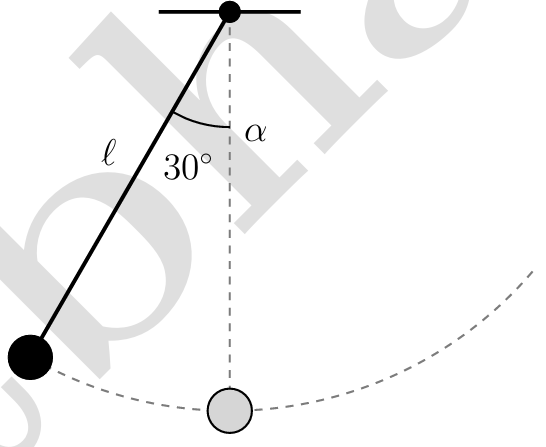
\includegraphics[width=0.32\textwidth]{images/8/8-8.png}\hfill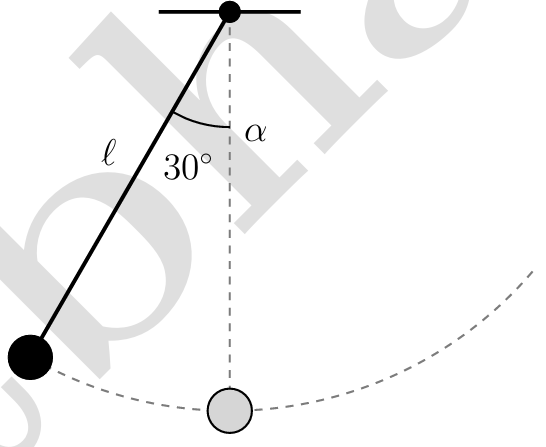
\includegraphics[width=0.32\textwidth]{images/8/8-9.png}\end{center}
\begin{pil}\item $4{,}31$ \item $6{,}69$ \item $48{,}49$ \item $2{,}39$ \item $7{,}43$\end{pil}
\end{soalbox}
\begin{pembox}{19}
Gunakan prinsip energi dengan memperhitungkan usaha gaya nonkonservatif. Penurunan ketinggian dari sudut $30^\circ$ ke titik terendah: $h=L(1-\cos30^\circ)$. Dengan $L=3{,}5$ m, $h=3{,}5\left(1-\tfrac{\sqrt3}{2}\right)\approx0{,}4699$ m. Energi potensial yang hilang $mgh=60(10)(0{,}4699)=281{,}9$ J. Lintasan busur $s=L\theta=3{,}5\left(\tfrac\pi6\right)=1{,}833$ m. Usaha gaya gesek $W_f=-fs=-60(1{,}833)=-110{,}0$ J. Energi kinetik di titik terendah $\tfrac12mv^2=mgh+W_f=281{,}9-110{,}0=171{,}9$ J. Maka $v=\sqrt{\dfrac{2(171{,}9)}{60}}\approx2{,}39$ m/s.
\jw{D}
\end{pembox}

\begin{soalbox}{20}{Superposisi Getaran Harmonik}
Dua getaran harmonik dengan frekuensi sudut yang sama dinyatakan oleh $y_1=6\sin20t$ dan $y_2=8\cos20t$, dengan $y$ dalam cm dan $t$ dalam sekon. Jika resultannya ditulis sebagai $y=R\sin(20t+\phi)$, maka amplitudo resultan $R$ adalah $\ldots$
\begin{pil}\item $14$ cm \item $12$ cm \item $10$ cm \item $8$ cm \item $2$ cm\end{pil}
\end{soalbox}
\begin{pembox}{20}
Getaran sin dan cos dengan frekuensi sama dapat dipandang sebagai dua komponen fasor yang berbeda fase $90^\circ$. Karena saling tegak lurus, amplitudo resultan $R=\sqrt{6^2+8^2}=\sqrt{100}=10$ cm.
\jw{C}
\end{pembox}

\begin{soalbox}{21}{Efek Doppler pada Bunyi Pantul}
Sebuah mobil pemadam bergerak menuju dinding sambil membunyikan sirene berfrekuensi $680$ Hz. Pengemudi mendengar bunyi pantul dari dinding dengan frekuensi $760$ Hz. Jika cepat rambat bunyi di udara $340$ m/s, kelajuan mobil pemadam adalah $\ldots$
\begin{pil}\item $54$ km/jam \item $60$ km/jam \item $68$ km/jam \item $72$ km/jam \item $90$ km/jam\end{pil}
\end{soalbox}
\begin{pembox}{21}
Bunyi pantul mengalami dua tahap Doppler. Untuk pantulan pada dinding diam, frekuensi yang didengar pengemudi $f'=f\dfrac{v+u}{v-u}$ dengan $u$ kelajuan mobil. Substitusi: $760=680\dfrac{340+u}{340-u}$, atau $\dfrac{19}{17}=\dfrac{340+u}{340-u}$. Kalikan silang: $17(340+u)=19(340-u)\Rightarrow 36u=680\Rightarrow u=18{,}89$ m/s. Konversi: $u=18{,}89(3{,}6)=68{,}0$ km/jam.
\jw{C}
\end{pembox}

\begin{soalbox}{22}{Gerak Rotasi Diperlambat}
Sebuah motor listrik yang dapat memutar roda dengan laju sudut $90$ putaran per menit dimatikan dengan perlambatan sudut sebesar $2$ rad/s$^2$. Lama waktu yang diperlukan roda tersebut untuk berhenti adalah $\ldots$ s.
\begin{pil}\item $6{,}17$ \item $4{,}71$ \item $2{,}09$ \item $6{,}23$ \item $5{,}24$\end{pil}
\end{soalbox}
\begin{pembox}{22}
Ubah kecepatan sudut awal: $90$ rpm $=\dfrac{90}{60}=1{,}5$ putaran/s. Karena satu putaran $2\pi$ rad, $\omega_0=1{,}5(2\pi)=3\pi$ rad/s. Dengan $\omega=\omega_0-\alpha t$ dan $\omega=0$: $t=\dfrac{\omega_0}{\alpha}=\dfrac{3\pi}{2}=4{,}71$ s.
\jw{B}
\end{pembox}

\begin{soalbox}{23}{Susunan Pegas dan Frekuensi}
Tiga pegas identik masing-masing berkonstanta $k$ disusun menjadi dua sistem. Sistem P terdiri atas dua pegas yang disusun seri lalu diparalelkan dengan satu pegas. Sistem Q terdiri atas dua pegas yang disusun paralel lalu diserikan dengan satu pegas. Kedua sistem dipasangi massa yang sama $m$. Perbandingan frekuensi getar sistem P dan Q, yaitu $f_P:f_Q$, adalah $\ldots$
\begin{pil}\item $1:2$ \item $\sqrt2:1$ \item $3:2$ \item $2:3$ \item $1:\sqrt2$\end{pil}
\end{soalbox}
\begin{pembox}{23}
Frekuensi sistem pegas-massa $f=\dfrac{1}{2\pi}\sqrt{\dfrac{k_{\text{eq}}}{m}}$. Karena massa sama, perbandingan frekuensi bergantung pada akar perbandingan konstanta ekuivalen. Sistem P: dua pegas seri $k_s=\dfrac{k\cdot k}{k+k}=\dfrac k2$, diparalelkan dengan $k$: $k_P=\dfrac k2+k=\dfrac{3k}{2}$. Sistem Q: dua pegas paralel $k_p=2k$, diserikan dengan $k$: $k_Q=\dfrac{(2k)(k)}{2k+k}=\dfrac{2k}{3}$. Maka $\dfrac{f_P}{f_Q}=\sqrt{\dfrac{k_P}{k_Q}}=\sqrt{\dfrac{3k/2}{2k/3}}=\sqrt{\dfrac94}=\dfrac32$.
\jw{C}
\end{pembox}

\begin{soalbox}{24}{Cepat Rambat Bunyi dalam Fluida}
Cepat rambat bunyi dalam fluida ideal memenuhi hubungan $v=\sqrt{B/\rho}$, dengan $B$ modulus bulk dan $\rho$ massa jenis fluida. Tinjau pernyataan berikut:
\begin{enumerate}[label=(\arabic*),leftmargin=*,topsep=2pt,itemsep=1pt]
\item Semakin besar modulus bulk, bunyi merambat semakin cepat.
\item Untuk $B$ tetap, semakin besar massa jenis maka bunyi merambat semakin lambat.
\item Tegangan permukaan merupakan besaran utama yang menentukan cepat rambat bunyi di seluruh fluida homogen.
\item Fluida yang sukar dimampatkan cenderung memiliki cepat rambat bunyi lebih besar.
\end{enumerate}
Pernyataan yang benar adalah $\ldots$
\begin{pil}\item (1) dan (2) \item (1), (2), dan (4) \item (2) dan (3) \item (3) dan (4) \item (1), (2), (3), dan (4)\end{pil}
\end{soalbox}
\begin{pembox}{24}
Dari $v=\sqrt{B/\rho}$, cepat rambat berbanding lurus dengan akar modulus bulk dan berbanding terbalik dengan akar massa jenis. Pernyataan (1) benar; (2) benar; (3) tidak tepat karena cepat rambat bunyi pada fluida homogen ideal terutama ditentukan oleh modulus bulk dan massa jenis, bukan tegangan permukaan; (4) benar karena fluida yang sukar dimampatkan memiliki modulus bulk besar. Jadi yang benar (1), (2), dan (4).
\jw{B}
\end{pembox}

\begin{soalbox}{25}{Pusat Massa Empat Benda}
Tinjau empat benda bermassa sama, dinamakan benda 1, 2, 3, dan 4. Benda $n$, dengan $n=1,2,3,4$, bergerak dengan vektor posisi $\vec r_n(t)=\dfrac n2\vec v+\vec a\,t$. Jika $\vec v=(4\hat i+2\hat j)$ m/s, $\vec a=-5\hat j$ m/s$^2$, dan pada $t=0$ s keempat benda berada di pusat koordinat, vektor posisi pusat massa sistem pada saat $t=1$ s adalah $\ldots$ m.
\begin{pil}\item $2\hat i-4\hat j$ \item $5\hat i-2{,}5\hat j$ \item $1{,}5\hat i-4{,}25\hat j$ \item $2{,}5\hat i-3{,}75\hat j$ \item $0{,}5\hat i-4{,}75\hat j$\end{pil}
\end{soalbox}
\begin{pembox}{25}
Karena keempat benda bermassa sama, posisi pusat massa adalah rata-rata posisi: $\vec r_{\text{PM}}=\dfrac{\vec r_1+\vec r_2+\vec r_3+\vec r_4}{4}$. Pada $t=1$ s, $\vec r_n(1)=\dfrac n2\vec v+\vec a$. Rata-rata $\dfrac n2$ untuk $n=1,2,3,4$ adalah $\dfrac{\tfrac12+1+\tfrac32+2}{4}=\dfrac54=1{,}25$. Maka $\vec r_{\text{PM}}=1{,}25\vec v+\vec a=1{,}25(4\hat i+2\hat j)-5\hat j=5\hat i+2{,}5\hat j-5\hat j=5\hat i-2{,}5\hat j$.
\jw{B}
\end{pembox}

\begin{soalbox}{26}{Efek Doppler Pengamat Menjauh}
Sebuah drone diam membunyikan alarm berfrekuensi $500$ Hz. Seorang pelari bergerak menjauhi drone dengan kelajuan $10$ m/s. Jika cepat rambat bunyi di udara $340$ m/s, frekuensi yang didengar pelari adalah $\ldots$
\begin{pil}\item $470{,}6$ Hz \item $485{,}3$ Hz \item $500{,}0$ Hz \item $514{,}7$ Hz \item $529{,}4$ Hz\end{pil}
\end{soalbox}
\begin{pembox}{26}
Sumber diam, pengamat menjauhi sumber, frekuensi yang didengar lebih kecil: $f'=f\dfrac{v-v_o}{v}$ dengan $v_o$ kelajuan pengamat. Substitusi: $f'=500\dfrac{340-10}{340}=500\dfrac{330}{340}=485{,}3$ Hz.
\jw{B}
\end{pembox}

\begin{soalbox}{27}{Periode Osilasi dari Energi Potensial}
Sebuah benda bermassa $2$ kg berosilasi harmonik sederhana pada pegas licin. Energi potensial sistem terhadap simpangan memenuhi hubungan $U=25x^2$, dengan $U$ dalam joule dan $x$ dalam meter. Periode osilasi benda tersebut adalah $\ldots$
\begin{pil}\item $\pi/10$ s \item $\pi/5$ s \item $\pi/\sqrt2$ s \item $2\pi/5$ s \item $\pi$ s\end{pil}
\end{soalbox}
\begin{pembox}{27}
Energi potensial pegas $U=\tfrac12kx^2$. Dari $U=25x^2$: $\tfrac12k=25\Rightarrow k=50$ N/m. Periode $T=2\pi\sqrt{\dfrac mk}=2\pi\sqrt{\dfrac{2}{50}}=2\pi\sqrt{\dfrac{1}{25}}=2\pi\left(\dfrac15\right)=\dfrac{2\pi}{5}$ s.
\jw{D}
\end{pembox}

\begin{soalbox}{28}{Pernyataan tentang Getaran Pegas}
Sebuah pegas yang dibebani bergetar vertikal sebanyak $15$ kali dalam $12$ sekon. Tinjau pernyataan berikut:
\begin{enumerate}[label=(\arabic*),leftmargin=*,topsep=2pt,itemsep=1pt]
\item Periode getaran adalah $0{,}8$ s.
\item Frekuensi getaran adalah $1{,}25$ Hz.
\item Waktu dari titik setimbang ke simpangan maksimum adalah $0{,}20$ s.
\item Percepatan maksimum terjadi saat beban berada di titik setimbang.
\end{enumerate}
Pernyataan yang benar adalah $\ldots$
\begin{pil}\item (1), (2), dan (3) \item (1) dan (3) \item (2) dan (4) \item (4) saja \item (1), (2), (3), dan (4)\end{pil}
\end{soalbox}
\begin{pembox}{28}
Frekuensi $f=\dfrac Nt=\dfrac{15}{12}=1{,}25$ Hz, jadi (2) benar. Periode $T=\dfrac1f=\dfrac{1}{1{,}25}=0{,}8$ s, jadi (1) benar. Waktu dari titik setimbang ke simpangan maksimum adalah seperempat periode: $\dfrac T4=\dfrac{0{,}8}{4}=0{,}20$ s, jadi (3) benar. Percepatan pada GHS $a=-\omega^2x$, maksimum saat $|x|$ maksimum yaitu di simpangan maksimum, bukan di titik setimbang, jadi (4) salah. Maka yang benar (1), (2), dan (3).
\jw{A}
\end{pembox}

\begin{soalbox}{29}{Tegangan Tali dari Persamaan Gelombang}
Sebuah gelombang transversal pada tali dinyatakan oleh $y=0{,}04\sin(\pi x-40\pi t)$, dengan $x$ dan $y$ dalam meter serta $t$ dalam sekon. Jika massa jenis linear tali adalah $2\times10^{-3}$ kg/m, maka tegangan tali adalah $\ldots$
\begin{pil}\item $1{,}6$ N \item $2{,}4$ N \item $3{,}2$ N \item $4{,}0$ N \item $6{,}4$ N\end{pil}
\end{soalbox}
\begin{pembox}{29}
Bentuk umum $y=A\sin(kx-\omega t)$, sehingga $k=\pi$ rad/m dan $\omega=40\pi$ rad/s. Cepat rambat $v=\dfrac\omega k=\dfrac{40\pi}{\pi}=40$ m/s. Untuk gelombang pada tali $v=\sqrt{\dfrac T\mu}$, maka $T=\mu v^2=(2\times10^{-3})(40)^2=(2\times10^{-3})(1600)=3{,}2$ N.
\jw{C}
\end{pembox}

\begin{soalbox}{30}{Usaha dan Energi pada Bidang Miring Licin}
Sebuah balok bermassa $4$ kg ditarik menggunakan gaya konstan $24$ N sehingga mendaki bidang miring licin. Gaya tersebut sejajar dengan permukaan bidang. Jika bidang miring membentuk sudut $30^\circ$ terhadap horizontal, percepatan gravitasi $g=10$ m/s$^2$, dan balok ditarik dari keadaan tak bergerak, kelajuan balok setelah mendaki bidang miring sejauh $2$ m adalah $\ldots$ m/s.
\begin{pil}\item $2{,}83$ \item $2{,}00$ \item $4{,}00$ \item $5{,}66$ \item $3{,}74$\end{pil}
\end{soalbox}
\begin{pembox}{30}
Bidang miring licin, gaya sepanjang bidang adalah gaya tarik ke atas dan komponen berat ke bawah. Komponen berat $mg\sin30^\circ=4(10)\left(\tfrac12\right)=20$ N. Gaya tarik $24$ N, sehingga resultan $\Sigma F=24-20=4$ N. Percepatan $a=\dfrac{\Sigma F}{m}=\dfrac44=1$ m/s$^2$. Balok mula-mula diam dan menempuh $s=2$ m. Dengan $v^2=v_0^2+2as=2(1)(2)=4$, maka $v=2$ m/s.
\jw{B}
\end{pembox}

%================= KUNCI JAWABAN =================
\clearpage
\begin{center}{\Large\bfseries Kunci Jawaban Ringkas}\end{center}
\medskip
\begin{center}
\renewcommand{\arraystretch}{1.3}
\begin{tabular}{*{10}{c}}
\textbf{1} E & \textbf{2} E & \textbf{3} A & \textbf{4} C & \textbf{5} B & \textbf{6} D & \textbf{7} D & \textbf{8} A & \textbf{9} B & \textbf{10} B\\
\textbf{11} C & \textbf{12} C & \textbf{13} E & \textbf{14} C & \textbf{15} C & \textbf{16} B & \textbf{17} B & \textbf{18} C & \textbf{19} D & \textbf{20} C\\
\textbf{21} C & \textbf{22} B & \textbf{23} C & \textbf{24} B & \textbf{25} B & \textbf{26} B & \textbf{27} D & \textbf{28} A & \textbf{29} C & \textbf{30} B\\
\end{tabular}
\end{center}
\vfill
\begin{center}\small\textbf{Follow TikTok: www.tiktok.com/@result\_han}\\\textbf{Paket soal PTN lainnya: lynk.id/result\_han}\end{center}

\end{document}
